\chapter{Alternative Measures of Clearance Time}\label{analysis}

\section{Alternative endpoints}
\subsection{PC50 and PC99}
\subsubsection*{PC50}
PC50 was estimated by log-linear interpolation. The PC50 clearance times thus obtained are plotted in Figure \ref{pc50anova} by experimental factors with sub-plots to look for interactions.
\begin{figure}[p]
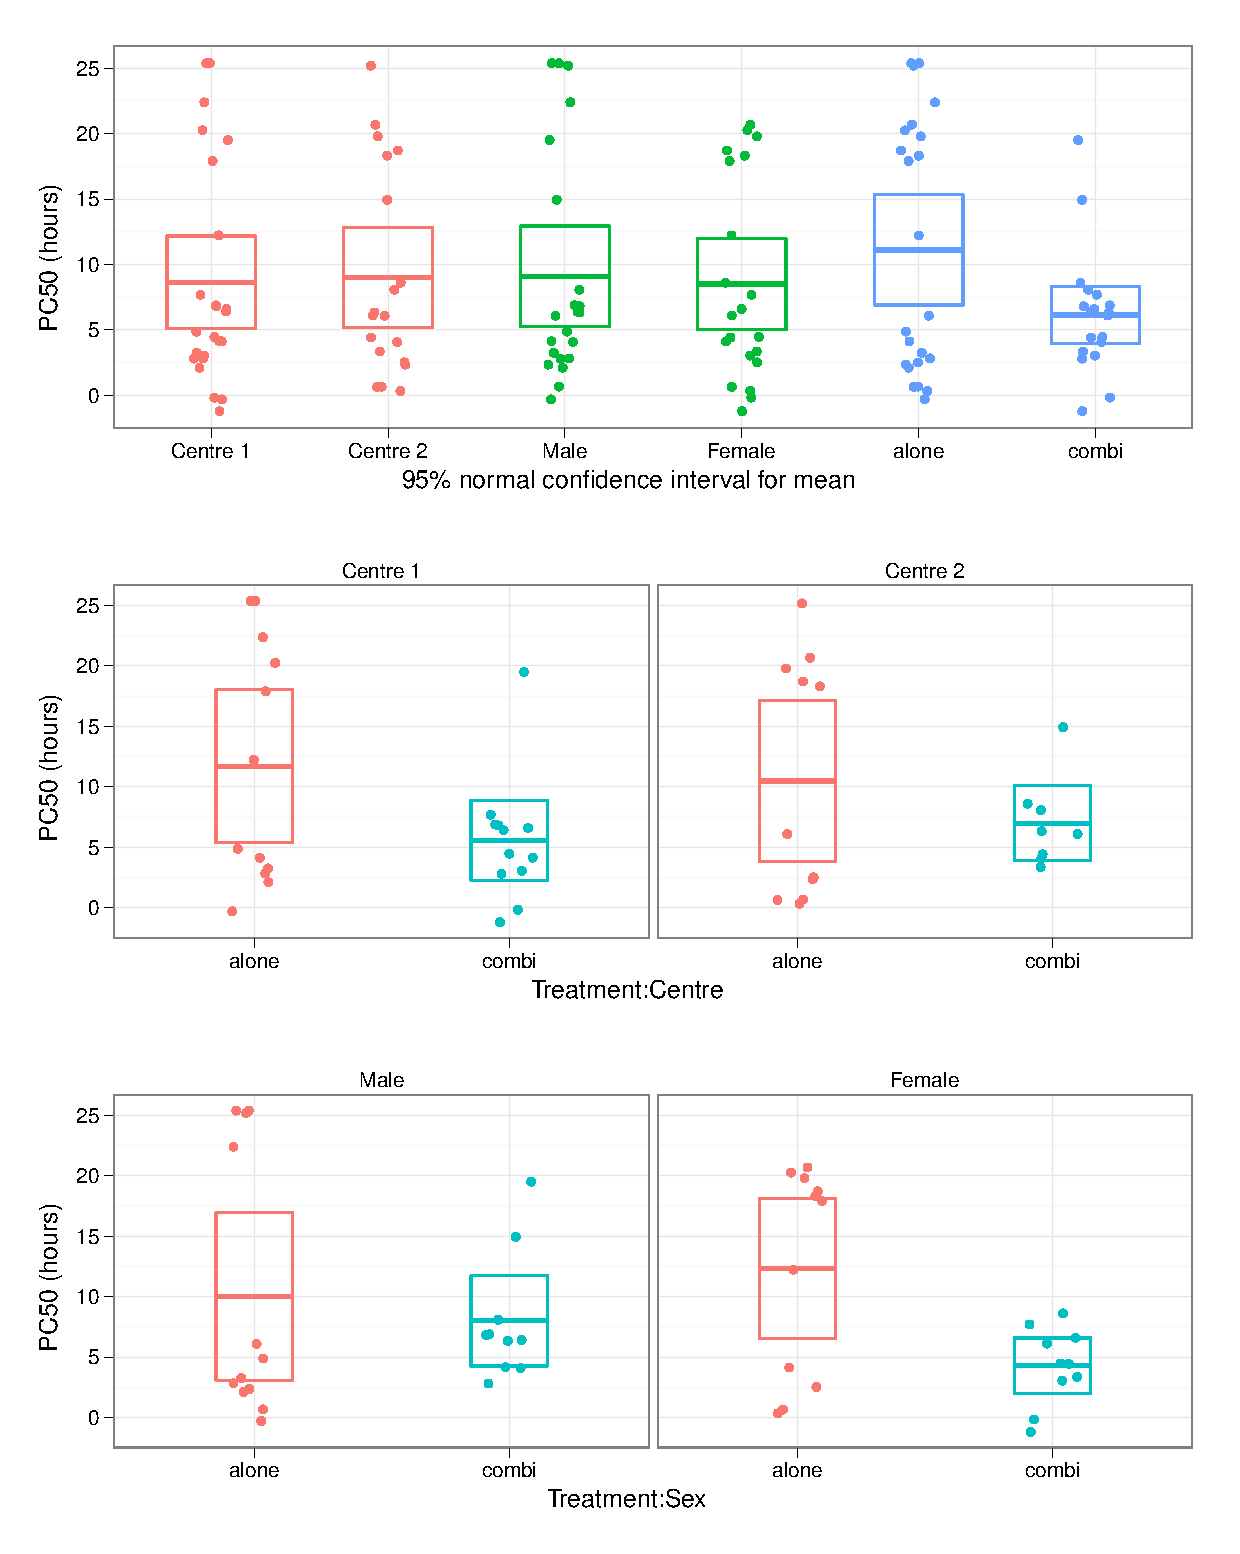
\includegraphics[width=150mm]{pc50anova.eps} 
\caption{Comparison of PC50 main effects and interactions with $t$ distribution 95\% confidence intervals for the means}
\label{pc50anova}
\end{figure}
A similar pattern can be seen as for PC90 (Figures \ref{pc90boxes} and \ref{pc90interaction} on pages \pageref{pc90boxes} and \pageref{pc90interaction}). The same key features are present namely
\begin{itemize}
\item No difference between centres.
\item A reduction in clearance time with the combined treatment, but only for female subjects.
\item A greater variance for subjects on the single (``alone'') treatment.
\end{itemize}

The same procedure of inspecting the distribution of standardized residuals was followed for choosing an appropriate ANOVA model for the data. As with PC90 it was found that the most suitable model for the PC50 clearance time was a 2-way ANOVA model by sex and treatment with a square-root transformation of the dependent variable, fitted by weighted least-squares, using the variances of the two treatment groups as the weighting. The results are shown in Table \ref{aov50}.
%> summary(PC50.loglin2rwt.aov)
%              Df Sum Sq Mean Sq F value  Pr(>F)  
%Sex            1  1.104   1.104  1.1652 0.28702  
%Treatment      1  2.089   2.089  2.2055 0.14556  
%Sex:Treatment  1  3.010   3.010  3.1771 0.08246 .
%Residuals     39 36.949   0.947
\begin{table}[h]
\centering
\caption{ANOVA table for PC50 model}\label{aov50}
\begin{tabular}{l|rrrrrl}
Source&Sum Sq.&df&Mean Sq.&$F$&P($>F$)\\
\hline
$Sex$				& 1.10 & 1 & 1.10 & 1.17 & 0.287 & \\
$Treatment$			& 2.09   & 1 & 2.09   & 2.21   & 0.146 & \\
$Sex\times Treatment$	& 3.01   & 1 & 3.01   & 3.18   & 0.082 & \\
$Residuals$			& 36.95 & 39 & 0.947 &&&\\
\hline
Total&43.15&42&&&
\end{tabular}
\end{table}

Although Figure \ref{pc50anova} seems to show a sex-treatment interaction effect on clearance times we do not have evidence at the 5\% level to reject the hypothesis that there is no effect of sex or treatment. This is probably because the difference between clearance times is smaller than for PC90 and we don't have enough data to detect this difference at the 5\% level.

The mean PC50 clearance times and confidence intervals are shown in Table \ref{inference50}.
\begin{table}[h]
\centering
\caption{Mean PC50 clearance times by sex and treatment}\label{inference50}
\begin{tabular}{|l|c|c|}
\hline
&Clearance time PC50&95\% conf. int.\\
Factor levels&(hrs:mins)&(hrs:mins)\\
\hline
Male, single treatment 		& 6:47 & (2:37, 12:54) \\
Female, single treatment		& 10:02 & (4:34,  17:37) \\
Male, combined treatment	& 7:22 & (3:50, 12:03) \\
Female, combined treatment	& 2:54 & (0:54, 6:03) \\
\hline
\end{tabular}
\end{table}

For female subjects the mean decrease in PC50 in the combined treatment group over the single treatment group is 7.1 hours with a 95\% confidence interval of (0.7, 9.9) hours.

\subsubsection*{PC99}
The log-linear interpolated PC99 values are plotted in Figure \ref{pc99anova}.
\begin{figure}[p]
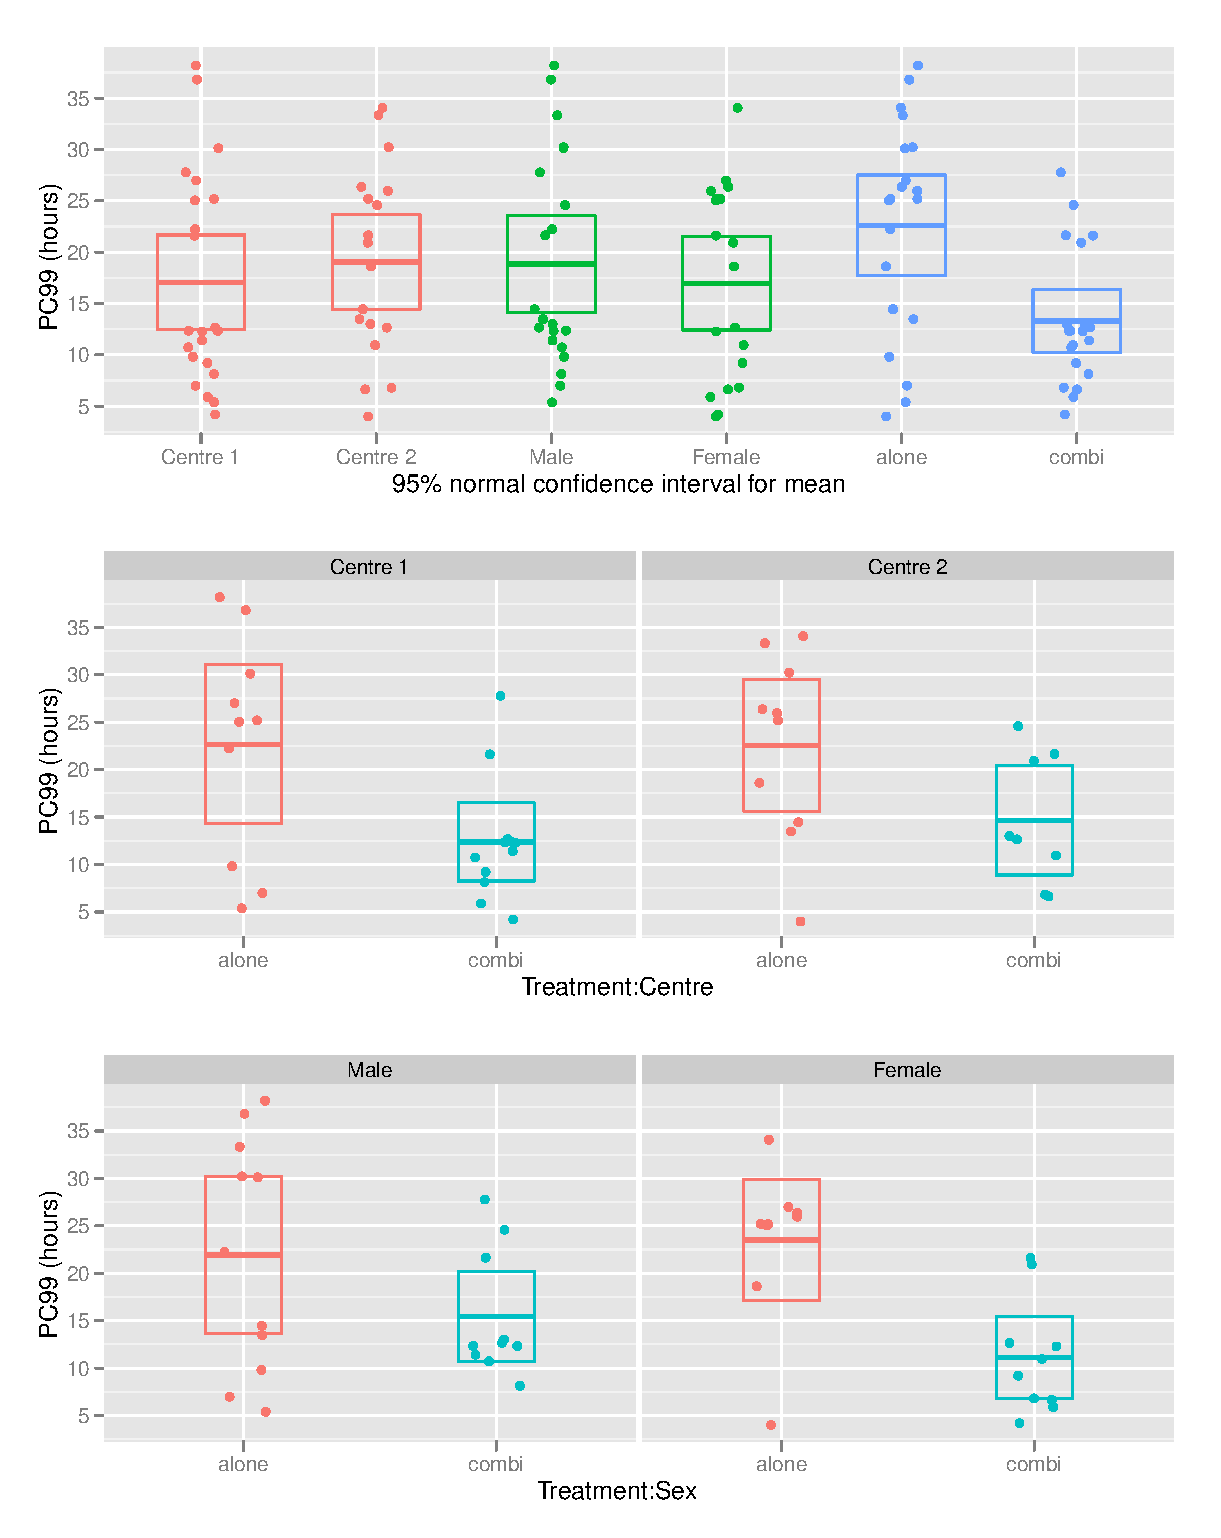
\includegraphics[width=150mm]{pc99anova.eps} 
\caption{Comparison of PC99 main effects and interactions with $t$ distribution 95\% confidence intervals for the means}
\label{pc99anova}
\end{figure}
For 3 subjects the parasite count did not reach the PC99 level by the end of the study, hence there is only PC99 data for 40 out of the 43 subjects. Once again there is no discernible effect of centre or sex alone on the clearance times. However, now the improvement of the combined treatment over the single treatment seems more symmetrical between sexes. Results of 2-way ANOVA by sex and treatment on the square-root transformed clearance times fitted by treatment-weighted least-squares are shown in Table \ref{aov99}.
%              Df Sum Sq Mean Sq F value   Pr(>F)   
%Sex            1  1.436   1.436  1.4664 0.233808   
%Treatment      1  9.074   9.074  9.2688 0.004339 **
%Sex:Treatment  1  1.643   1.643  1.6781 0.203416   
%Residuals     36 35.243   0.979              
\begin{table}[h]
\centering
\caption{ANOVA table for PC99 model}\label{aov99}
\begin{tabular}{l|rrrrrl}
Source&Sum Sq.&df&Mean Sq.&$F$&P($>F$)\\
\hline
$Sex$				& 1.44 & 1 & 1.44 & 1.47 & 0.234 & \\
$Treatment$			& 9.07   & 1 & 9.07   & 9.27   & 0.004 &** \\
$Sex\times Treatment$	& 1.64   & 1 & 1.64   & 1.68   & 0.203 & \\
$Residuals$			& 35.243 & 36 & 0.979 &&&\\
\hline
Total&47.40&39&&&
\end{tabular}\\
**$<0.005$
\end{table}

It can be seen that there is evidence to reject the hypothesis that treatment has no effect on PC99 clearance time, but no evidence to reject the hypothesis that sex has no effect. Therefore, we can exclude sex as a factor and refit a 1-way ANOVA model by treatment alone, giving the results shown in Table \ref{aov99r}.
%            Df Sum Sq Mean Sq F value  Pr(>F)   
%Treatment    1  9.396   9.396  9.3959 0.00399 **
%Residuals   38 38.000   1.000   
\begin{table}[h]
\centering
\caption{1-way ANOVA table for PC99 model}\label{aov99r}
\begin{tabular}{l|rrrrrl}
Source&Sum Sq.&df&Mean Sq.&$F$&P($>F$)\\
\hline
$Treatment$			& 9.40   & 1 & 9.40   & 9.40   & 0.004 &** \\
$Residuals$			& 38.0 & 38 & 1.00 &&&\\
\hline
Total&47.40&39&&&
\end{tabular}\\
**$<0.005$
\end{table}

The mean PC99 clearance time for patients on the single treatment is 21:07 (hrs:mins) with a 95\% confidence interval of (16:12, 26:41); for the combined treatment it is 12:33 (9:53, 15:32). This gives a mean decrease in PC99 for subjects on the combined treatment over the single treatment of 9.3 hours with a 95\% confidence interval of (3.7, 15.0) hours.

\subsection{Parasite reduction ratios}
Another endpoint used in studies of the efficacy of antimalarial drugs is the \emph{Parasite Reduction Ratio}, which is the ratio of the pre-dose parasite count to the count at a specific time from the time of first dose. 48 hours is often chosen as a time to calculate this ratio (PRR48) as this represents the reduction in parasites over a single lifecycle of the parasites\cite{white}. ``PRR24'', The reduction over 24 hours is also used\cite{newton}.

PRR48 measurements are not available for our data as the parasite count is 0 by 48 hours for all but 6 subjects. Even after 24 hours there are only 25 of the 43 subjects with non-zero parasite counts. After 12 hours though there are still 37 of the 43 subjects with a non-zero parasite count so we can look at PRR12 and have reasonable numbers in groups to make comparisons between treatments. The log parasite reduction ratio after 12 hours is shown in Figure \ref{prr12}
\begin{figure}
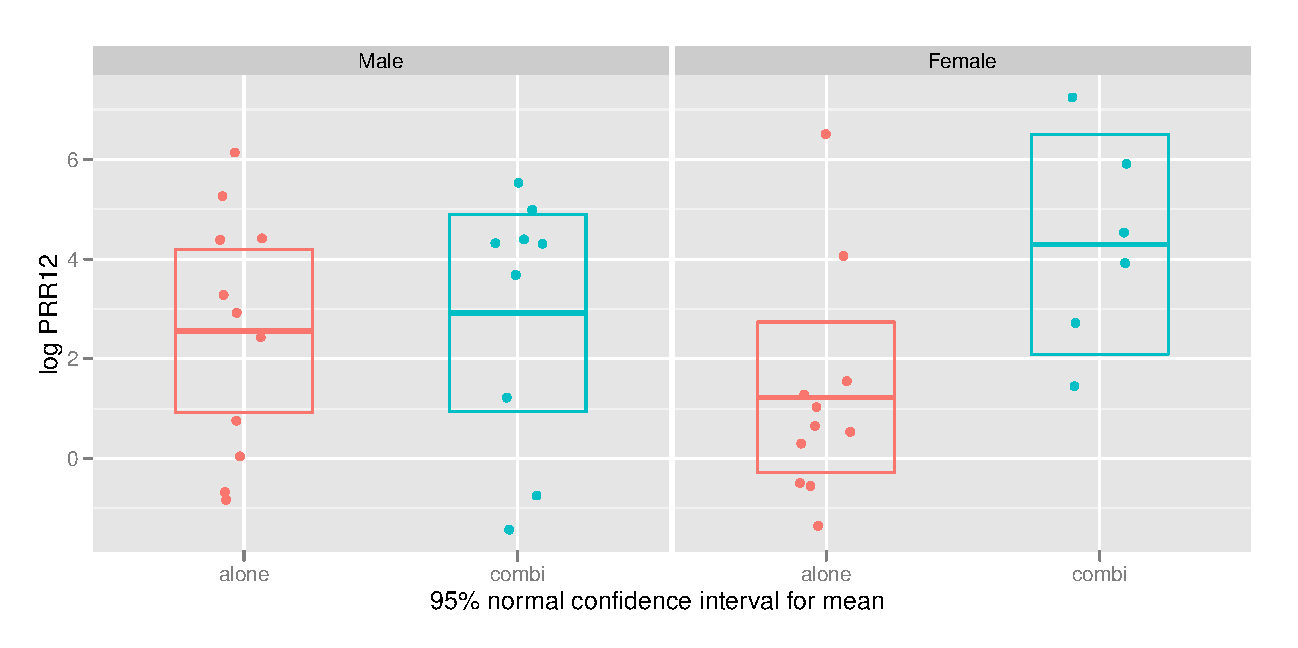
\includegraphics[width=150mm]{prr12.eps} 
\caption{log PRR12 with 95\% confidence intervals for the means}
\label{prr12}
\end{figure}

A similar pattern as with the PC90 and PC50 endpoints can be seen in that the treatment only seems to be effective among female patients in increasing PRR. It was found that a logarithmic transformation was appropriate for 2-way ANOVA modelling of the PRR12 data giving the results shown in Table \ref{aovprr12}.
%              Df  Sum Sq Mean Sq F value  Pr(>F)  
%Sex            1   1.524   1.524  0.2725 0.60512  
%Treatment      1  21.265  21.265  3.8024 0.05972 .
%Sex:Treatment  1  15.951  15.951  2.8521 0.10069  
%Residuals     33 184.557   5.593          
\begin{table}[h]
\centering
\caption{ANOVA table for PC99 model}\label{aovprr12}
\begin{tabular}{l|rrrrrl}
Source&Sum Sq.&df&Mean Sq.&$F$&P($>F$)\\
\hline
$Sex$				& 1.52 & 1 & 1.52 & 0.273 & 0.605 & \\
$Treatment$			& 21.27   & 1 & 21.27   & 3.80 & 0.060 & \\
$Sex\times Treatment$	& 15.95   & 1 & 15.95   & 2.85   & 0.101 & \\
$Residuals$			& 184.56 & 33 & 5.59 &&&\\
\hline
Total&223.30&36&&&
\end{tabular}
\end{table}

It can be seen that there is some evidence between the 5 and 10\% level to reject the hypothesis that the treatment has no effect on the parasite reduction ratio after 12 hours. It may be that we don't have enough data to detect the treatment effect observed in Figure \ref{prr12}. The model gives a mean increase in PRR12 for subjects on the combined treatment over those on the single treatment of 25.5 with a 95\% confidence interval of (-0.4, 159.8).

%\subsection{Logistic model of those cured after 24 hours?}

\section{Functional data analysis}
\begin{figure}[h]
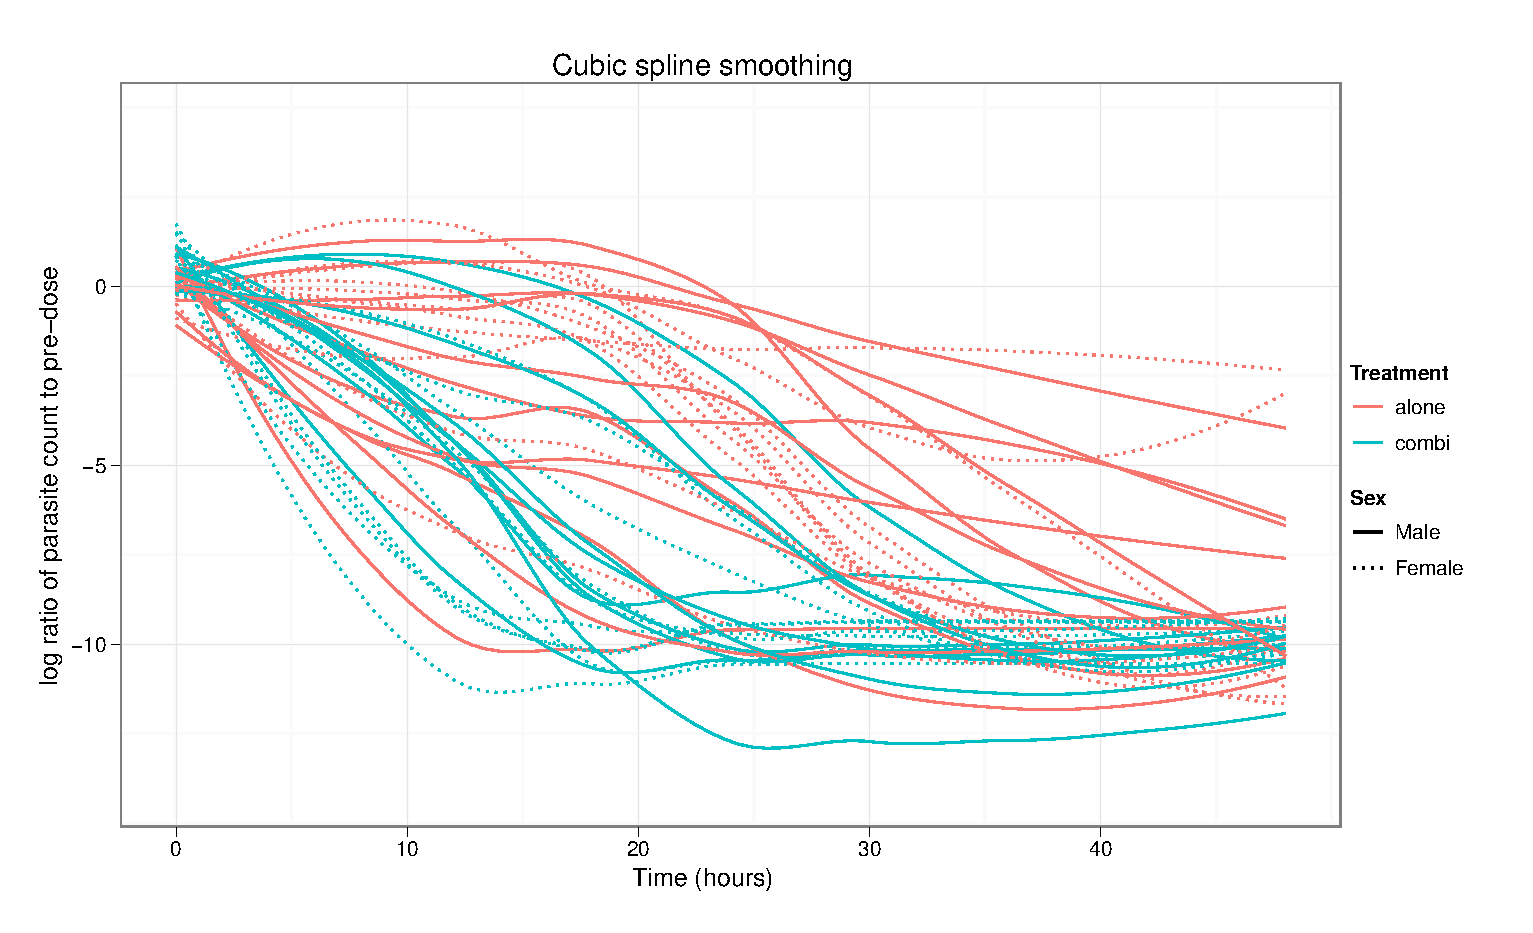
\includegraphics[width=150mm]{cubicspline.eps} 
\caption{}
\label{cubicspline}
\end{figure}
\begin{figure}[h]
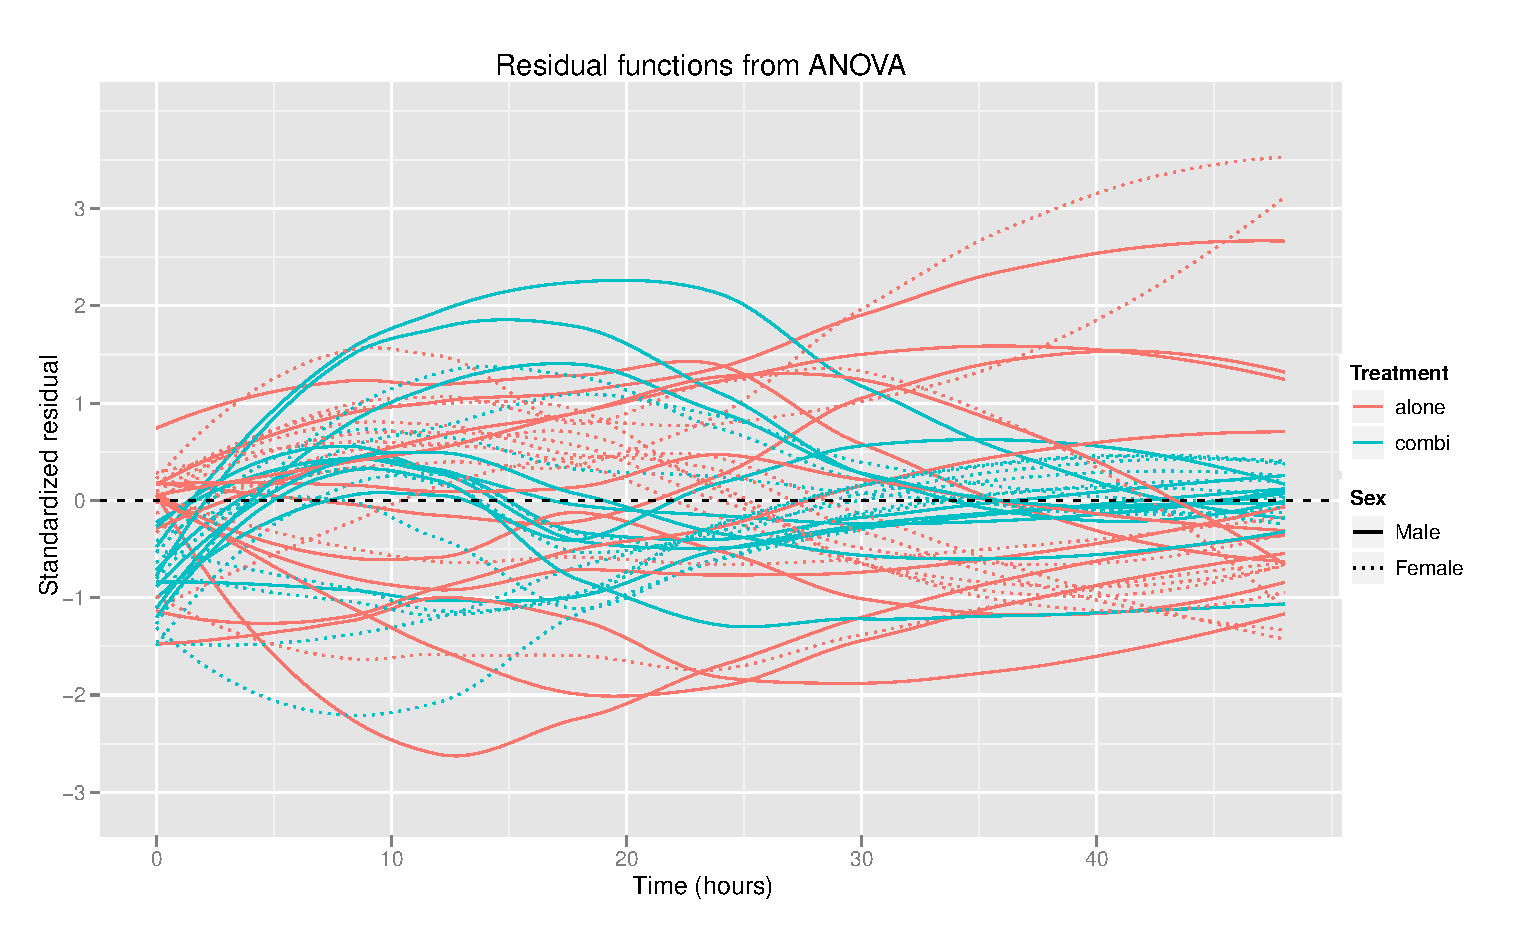
\includegraphics[width=150mm]{fdaresids.eps} 
\caption{}
\label{fdaresids}
\end{figure}
\begin{figure}[h]
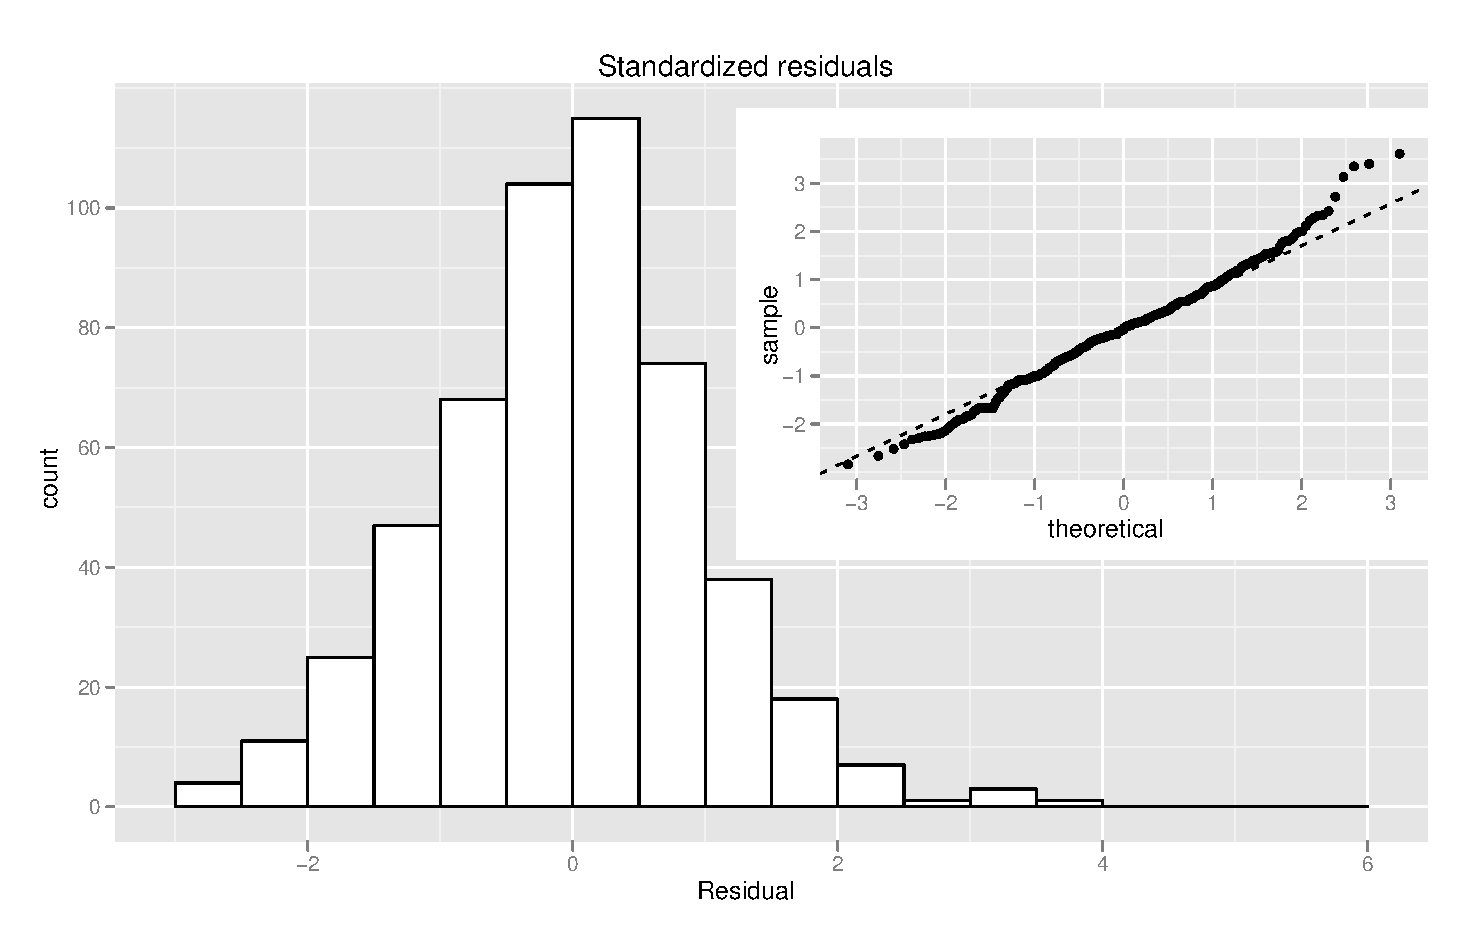
\includegraphics[width=150mm]{fdahistqq.eps} 
\caption{}
\label{fdahistqq}
\end{figure}
\begin{figure}[h]
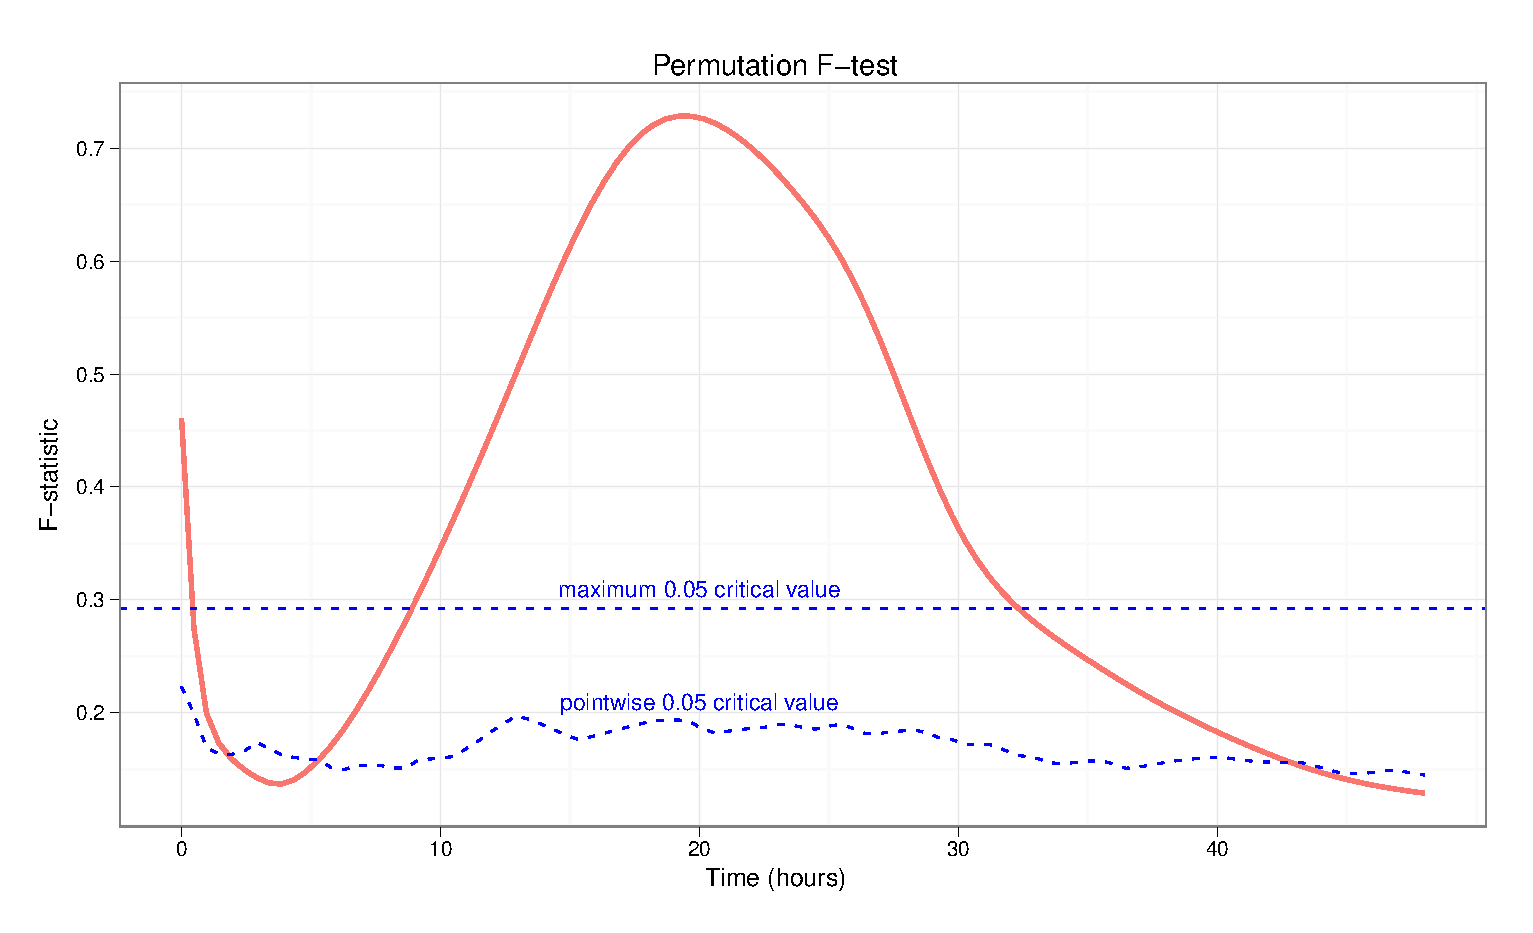
\includegraphics[width=150mm]{fdapermF.eps} 
\caption{}
\label{fdapermF}
\end{figure}
\begin{figure}[h]
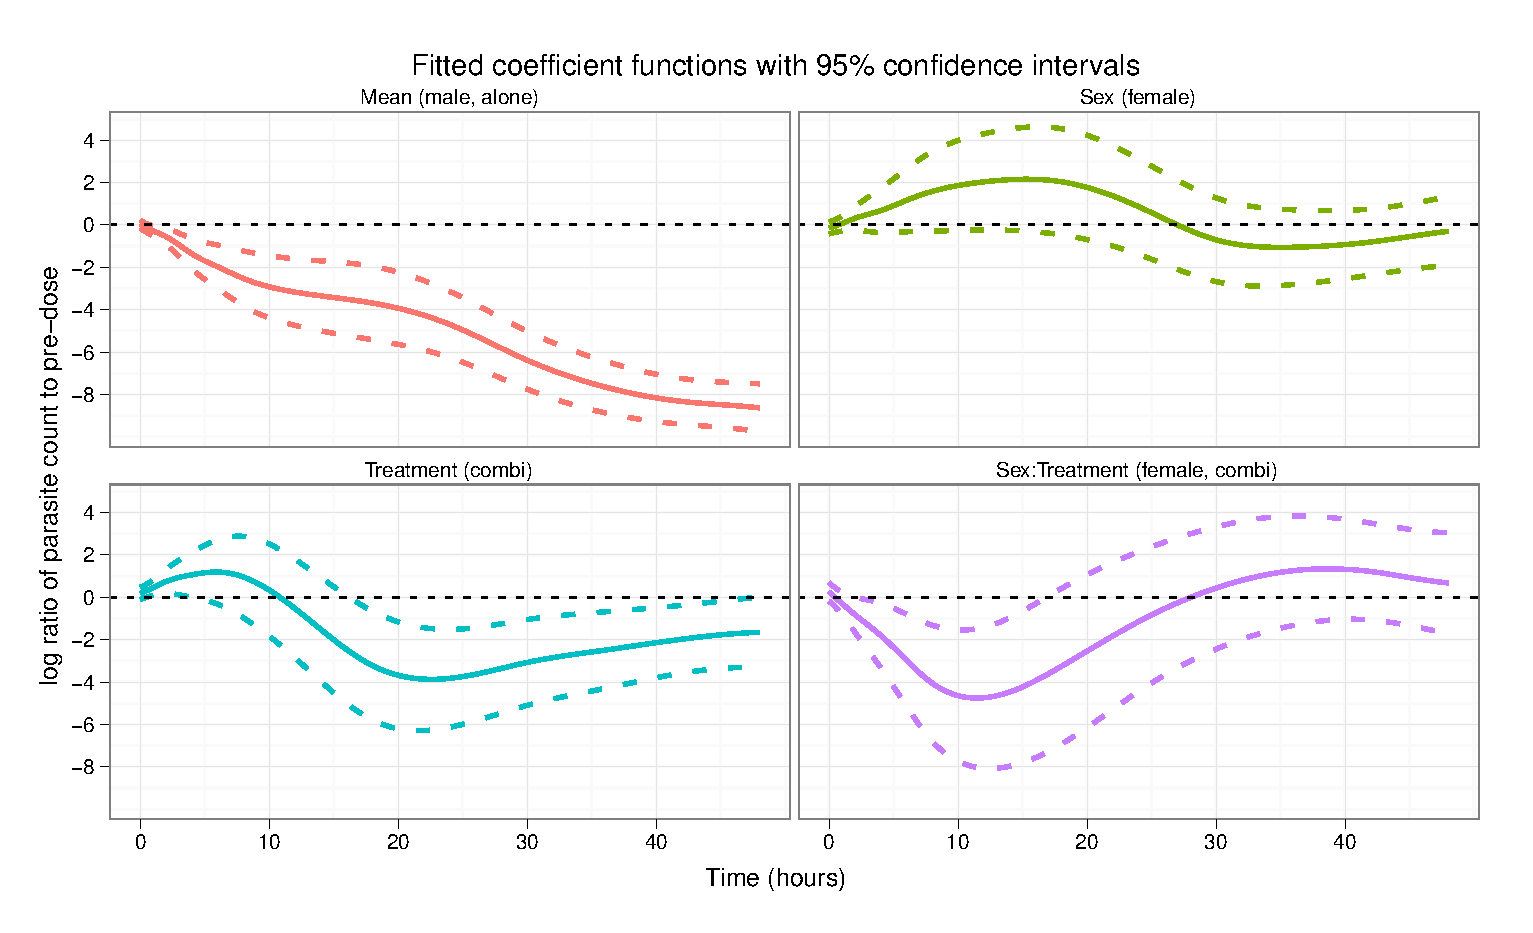
\includegraphics[width=150mm]{fdcoef.eps} 
\caption{}
\label{fdcoef}
\end{figure}
\begin{figure}[h]
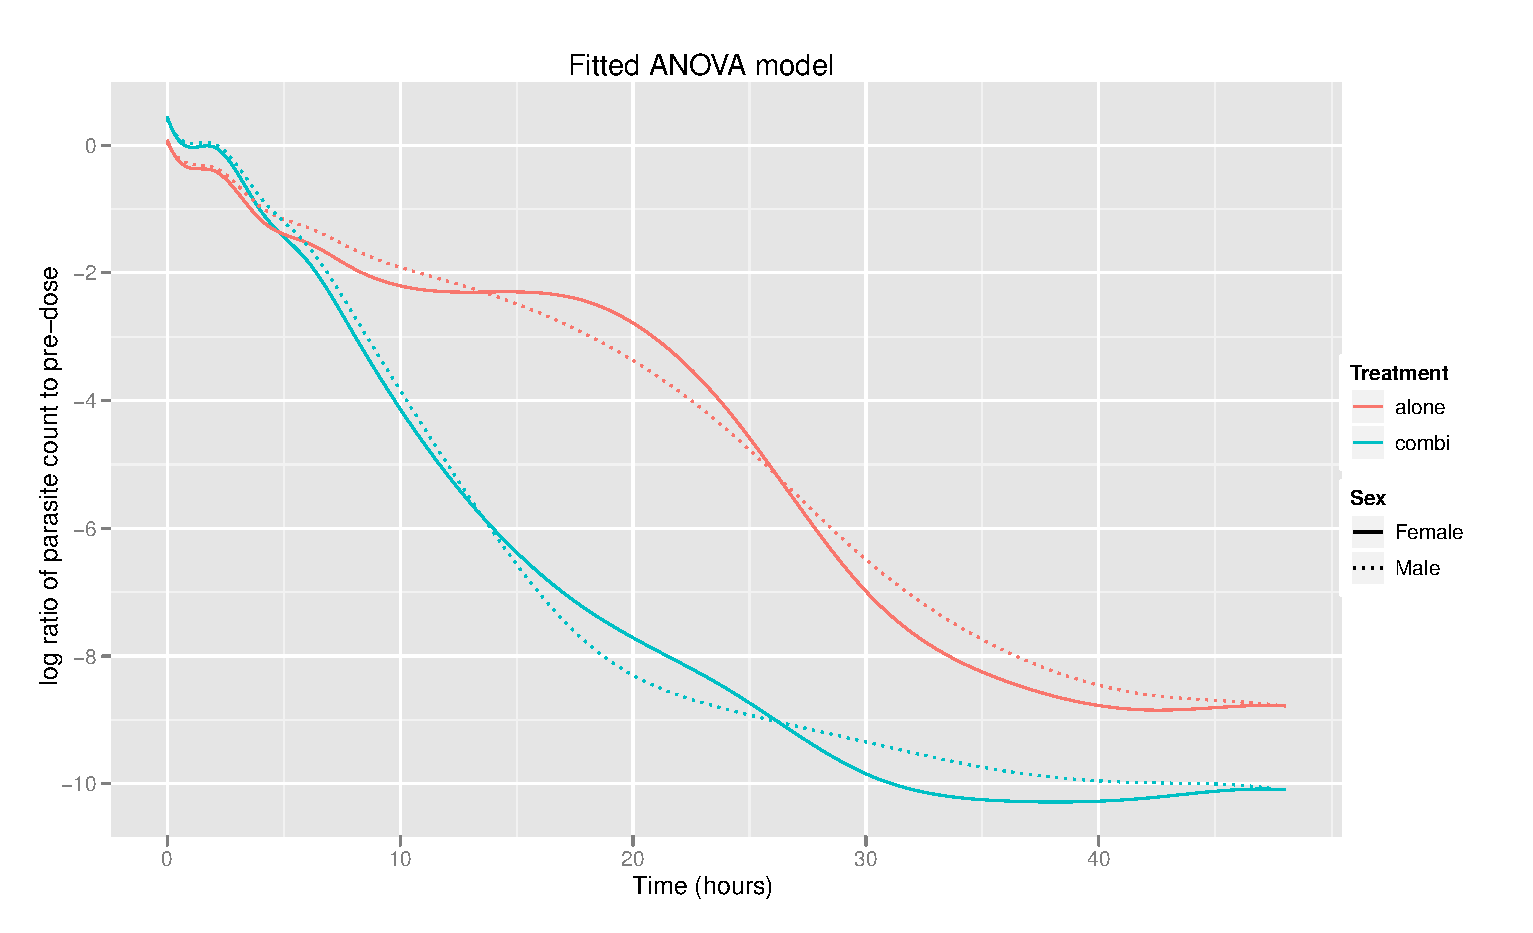
\includegraphics[width=150mm]{fdfitted.eps} 
\caption{}
\label{fdfitted}
\end{figure}

%\section{Key results}